\documentclass{myclass}
\usepackage[polish]{babel}

\title{Porównanie metod konstrukcji diagramu Woronoja}
\author{Bartosz Hanc, Jakub Pawlina}

\begin{document}

\maketitle
\tableofcontents

\subsection{Część techniczna}

Projekt został wykonany w środowisku Jupyter Notebook w języku Python z
wykorzystaniem dostarczonego na laboratoriach narzędzia graficznego. Wszystkie
dostępne funkcjonalności programu zostały opisane w notatniku Jupyter, natomiast
ich uruchomienie jest możliwe poprzez uruchomienie odpowiedniej komórki w
notatniku. Do implementacji samych algorytmów wykorzystano jedynie bibliotekę
standardową Pythona.

\subsubsection{Wprowadzanie danych wejściowych}

Danymi wejściowymi jest lista punktów reprezentowana przez pary typu
\texttt{(float, float)}. Oprócz bezpośredniego wpisania listy punktów możliwe
jest zadawanie punktów za pomocą myszki, korzystając z interfejsu graficznego.
Wprowadzone w taki sposób dane można następnie zapisać do pliku \texttt{.json}
poprzez uruchomienie odpowiedniej komórki. Możliwe jest następnie wczytanie
danych wejściowych z pliku \texttt{.json} korzystając z funkcji
\texttt{loadPoints("name.json")} przez podanie nazwy pliku znajdującego się w
tym samym folderze co notatnik Jupyter. Dodatkowo istnieje również opcja
wygenerowania \(n\) losowych punktów należących do zadanego obszaru płaszczyzny
\([a;b]\times[a;b]\) poprzez wywołanie funkcji
\texttt{genRndPoints(n,a,b)}.

\subsubsection{Wizualizacja wyników}

Notatnik Jupyter zawiera również zaimplementowane funkcje
\texttt{showResults1(points)} oraz \\ \texttt{showResults2(points)}
wizualizujące wyniki działania odpowiednio pierwszego i drugiego
zaimplementowanego algorytmu.

Dostępna jest również interaktywna wizualizacja algorytmu prezentująca
graficznie kolejne etapy jego działania. Wizualizację można uruchomić poprzez
uruchomienie odpowiedniej komórki w notatniku.

\subsection{Opis problemu}
\textbf{Diagramem Woronoja} generowanym przez zbiór punktów
\(S:=\{p_1,...,p_n\}\subset \mathbb{R}^2\) nazywamy podział płaszczyzny
\(\mathbb{R}^2\) na obszary \(H_1\),...,\(H_n\) parami rozłączne, takie że dla
każdego \(H_i\) zachodzi \(\forall_{p\in H_i}: d(p,p_i) = \min\left\{d(p,p_j) \,
| \, p_j\in S\right\} \),  gdzie \(d:\mathbb{R}^2\times\mathbb{R}^2\mapsto
\mathbb{R}_+\) jest metryką na płaszczyźnie \(\mathbb{R}^2\).

Celem projektu było zaimplementowanie dwóch różnych algorytmów wyznaczających diagram Woronoja zadanej chmury punktów na płaszczyźnie euklidesowej.

\subsection{Konstrukcja diagramu Woronoja jako grafu dualnego do triangulacji Delaunay'a wyznaczonej algorytmem Bowyera--Watsona}

\subsubsection{Opis algorytmu}

Jako jedną z dwóch wymaganych metod konstrukcji diagramów Woronoja wybrano
metodę konstrukcji korzystającą z dualności między triangulacją Delaunay'a, a
diagramem Woronoja. Schemat postępowania jest wówczas następujący: wyznaczamy
najpierw triangulację Delaunay'a chmury punktów, a następnie na jej podstawie
tworzymy krawędzie diagramu Woronoja. Do wyznaczenia triangulacji Delaunay'a
wykorzystano algorytm Bowyera--Watsona. Ideę zaproponowanej metody można
przedstawić w postaci elementarnego pseudokodu\footnote{Przedstawiony pseudokod
z niewielkimi modyfikacjami został zaczerpnięty z artykułu \href{https://en.wikipedia.org/wiki/Bowyer\%E2\%80\%93Watson_algorithm\#Pseudocode}{,,Bowyer--Watson algorithm''} na Wikipedii.}:

\begin{small}
\begin{verbatim}
    funkcja BowyerWatson:
        points := lista zadanych punktów
        triangles := pusty zbiór trójkątów triangulacji
        
        Znajdź super-prostokąt pokrywający całkowicie chmurę punktów.
        Dodaj do triangles dwa super-trójkąty powstałe z podziału 
        super-prostokąta jedną z jego przekątnych.
        
        Dla każdego punktu p z points:
            Znajdź wszystkie trójkąty T, takie że okrąg opisany na T zawiera 
            punkt p i dodaj je do zbioru badTriangles.
            
            Znajdź krawędzie wielokąta, który powstałby po usunięciu trójkątów 
            z badTriangles i dodaj je do zbioru polygon.
            
            Usuń z triangles wszystkie trójkąty znajdujące się w badTriangles.
            
            Dokonaj triangulacji powstałej wielokątnej wnęki polygon.
        
        Usuń z triangles wszystkie trójkąty, które zawierają wierzchołek 
        super-trójkąta.
        
        Oblicz diagram Woronoja jako graf dualny do triangulacji Delaunaya 
        zawartej w triangles.
\end{verbatim}
\end{small}

Dokładny opis implementacji w języku Python poszczególnych fragmentów powyższego
pseudokodu został opisany poniżej.
\begin{itemize}
    \item \textbf{Wykorzystane struktury danych}
    \begin{itemize}
        \item Wejściowe punkty są przechowywane w liście \texttt{points}, która
        zawiera pary typu \\\texttt{(float,float)} określające współrzędne
        kolejnych punktów
        
        \item Struktura \texttt{triangles} przechowuje trójki postaci
        \texttt{(int,int,int)} określające wierzchołki trójkąta jako indeksy
        punktów w liście \texttt{points}. Struktura \texttt{triangles} została
        zaimplementowana jako pythonowy \texttt{set()}.
        
        \item Struktura \texttt{edges} przechowuje pary typu key-value, gdzie
        kluczami są pary typu \texttt{(int,int)} określające krawędź
        triangulacji jako indeksy punktów w liście \texttt{points}, natomiast
        wartościami są zbiory zawierające trójkąty, które zawierają krawędź
        będąca kluczem. Trójkąty te są reprezentowane tak jak w strukturze
        \texttt{triangles} tj. w postaci trójek typu \texttt{(int,int,int)}.
        Struktura \texttt{edges} została zaimplementowana jako pythonowy
        słownik.
    \end{itemize}

    \item \textbf{Konstrukcja superprostokąta pokrywającego chmurę punktów.}
    Superprostokąt obliczamy poprzez znalezienie maksymalnej i minimalnej
    współrzędnej \(x\) i \(y\) chmury punktów, obliczenie wielkości
    \(l:=\max(|y_\text{max}-y_\text{min}|, |x_\text{max}-x_\text{min}|)\), a
    następnie odpowiednio dodanie i odjęcie \(l\) do/od \(x_\text{max}\),
    \(y_\text{max}\) i \(x_\text{min}\), \(y_\text{min}\). Parametr \(l\)
    określa wielkość obszaru, do którego ograniczamy obliczany diagram Woronoja.

    \item \textbf{Poszukiwanie trójkątów, których okrąg opisany zawiera dany
    punkt \(p\).} Dla każdego trójkąta \(T(A,B,C)\) znajdującego się aktualnie w
    zbiorze \texttt{triangles} obliczamy współrzędne \((S_x,S_y)\) środka okręgu
    opisanego na nim, korzystając ze wzorów
    \begin{equation*}
        \begin{split}
            &S_x = \frac{1}{D}\left[(A_x^2+A_y^2)(B_y-C_y)+(B_x^2+B_y^2)(C_y-A_y)+(C_x^2+C_y^2)(A_y-B_y)\right]\\
            &S_y = \frac{1}{D}\left[(A_x^2+A_y^2)(C_x-B_x)+(B_x^2+B_y^2)(A_x-C_x)+(C_x^2+C_y^2)(B_x-A_x)\right]
        \end{split}\quad,
    \end{equation*}
    gdzie \(D:=2[A_x(B_y-C_y)+B_x(C_y-A_y)+C_x(A_y-B_y)]\) oraz promień tego
    okręgu korzystając ze wzoru 
    \begin{equation*}
        R = \frac{abc}{4\sqrt{s(s-a)(s-b)(s-c)}}\,,
    \end{equation*}
    gdzie \(a\), \(b\), \(c\) to długości boków trójkąta, a
    \(s:=\frac{1}{2}(a+b+c)\). Jeśli odległość punktu \(p\) od środka
    \texttt{centre\((A,B,C)\)} jest mniejsza lub równa \(R\) to dodajemy trójkąt
    \(T(A,B,C)\) do zbioru \texttt{badTriangles} (\texttt{badTriangles} jest
    implementowany jako pythonowy \texttt{set()}). Równość sprawdzana jest przez
    warunek \(|\texttt{dist}(p,\texttt{centre}) - R| < \texttt{err}\), gdzie
    \texttt{err} to tolerancja dla zera.

    \item \textbf{Poszukiwanie krawędzi wielokątnej wnęki.} Dla każdego trójkąta
    \(T(A,B,C)\) znajdującego się w zbiorze \texttt{badTriangles} przypisujemy
    \(a, b, c = (A,B), (B,C), (C,A)\), a następnie dla każdej krawędzi \(e\) z
    \((a,b,c)\) obliczamy moc zbioru
    \((\texttt{edges}[e]\cap\texttt{badTriangles})-\{T\}\) (ponieważ
    \(\#\texttt{edges}[e]\leq2\) oraz złożoność znalezienia części wspólnej \(s
    \cap t\) to \(O(\min(\#s,\#t))\), a złożoność znalezienia różnicy \(s - t\)
    to \(O(\#s)\), więc obliczenie mocy zbioru w powyższy sposób zajmuje
    \(O(1)\) operacji). Jeśli moc powyższego zbioru wynosi 0 to dana krawędź
    \(e\) nie jest krawędzią wspólną żadnych dwóch trójkątów ze zbioru
    \texttt{badTriangles}, czyli jest krawędzią poszukiwanego wielokąta i
    dodajemy ją do zbioru krawędzi \texttt{polygon} (\texttt{polygon} jest
    implementowany jako pythonowy \texttt{set()})

    \item \textbf{Usuwanie nieprawidłowych trójkątów.} Dla każdego trójkąta
    \(T(A,B,C)\) znajdującego się w zbiorze \texttt{badTriangles} przypisujemy
    \(a, b, c = (A,B), (B,C), (C,A)\). Usuwamy \(T\) ze zbioru
    \texttt{triangles} korzystając z metody \texttt{.remove()} (o złożoności
    czasowej \(O(1)\)), a następnie aktualizujemy strukturę \texttt{edges}: dla
    każdej krawędzi \(e\) z \((a,b,c)\) usuwamy trójkąt \(T\) ze zbioru
    \(\texttt{edges}[e]\) korzystając z metody \texttt{.remove()} i jeśli po
    usunięciu zbiór ten jest pusty usuwamy klucz \(e\) ze słownika
    \texttt{edges} korzystając z metody \texttt{del} (o złożoności \(O(1)\)).

    \item \textbf{Triangulacja wielokątnej wnęki.} Dla każdej krawędzi \(e =
    (q,r)\) ze zbioru \texttt{polygon} dodajemy do zbioru \texttt{triangles}
    trójkąt \(T(p,q,r)\) i aktualizujemy strukturę \texttt{edges}: przypisujemy
    \(a, b, c = (p,q), (q,r), (r,p)\), a następnie dla każdej krawędzi \(e\) z
    \((a,b,c)\) wykonujemy:
    \begin{itemize}
        \item jeśli klucz \(e\) istnieje już w \texttt{edges} (sprawdzamy to w
        \(O(1)\), korzystając z metody \texttt{.get()}) to dodajemy do zbioru
        \(\texttt{edges}[e]\) trójkąt \(T(p,q,r)\);

        \item jeśli klucz \(e\) nie istnieje, to go tworzymy i wstawiamy do
        pustego zbioru \(\texttt{edges}[e]\) trójkąt \(T(p,q,r)\).
    \end{itemize}
    
    \item \textbf{Usuwanie trójkątów zawierających wierzchołek początkowego
    supertrójkąta.} Dla każdego trójkąta \(T(A,B,C)\) znajdującego się w zbiorze
    \texttt{triangles} sprawdzamy, czy \(A\) lub \(B\) lub \(C\) są
    wierzchołkami supertrójkąta. Jeśli tak to dodajemy \(T\) do zbioru
    \texttt{toRemove}. Następnie dla każdego trójkąta \(T\) ze zbioru
    \texttt{toRemove} usuwamy \(T\) ze zbioru \texttt{triangles} korzystając z
    metody \texttt{.remove()}.

    \item \textbf{Obliczenie diagramu Woronoja dualnego do wyznaczonej
    triangulacji Delaunay'a.} Diagram Woronoja jest reprezentowany przez listę
    \texttt{voronoi} zawierającą krawędzie go tworzące. Dla każdej krawędzi
    \(e\) będącej kluczem w \texttt{edges} przypisujemy \(\texttt{Ts} =
    \texttt{edges}[e] \cap \texttt{triangles}\) (\(O(1)\)). Jeśli
    \(\#\texttt{Ts} = 2\) to krawędź \(e\) jest krawędzią wspólną dwóch
    trójkątów \(T_1(A_1,B_1,C_1)\), \(T_2(A_2,B_2,C_2)\) zatem do listy
    \texttt{voronoi} dodajemy krawędź \([\texttt{centre}(A_1,B_1,C_1),
    \texttt{centre}(A_1,B_2,C_2)]\). Jeśli \(\#\texttt{Ts} = 1\) to krawędź
    \(e\) należy do otoczki wypukłej chmury punktów i krawędź diagramu Woronoja
    jest fragmentem prostej prostopadłej do \(e\). W celach wizualizacji możemy
    jednak utworzyć w tym przypadku krawędź pomiędzy trójkątem \(T_1\) z
    \texttt{Ts} i trójkątem \(T_2\) zawierającym wierzchołek supertrójkąta, przy
    czym oba trójkąty \(T_1\) i \(T_2\) znajdują się w zbiorze
    \(\texttt{edges}[e]\).

\end{itemize}

Ze względu na przeszukiwanie wszystkich trójkątów w strukturze
\texttt{triangles} w celu utworzenia zbioru \texttt{badTriangles} złożoność
czasowa opisanego algorytmu wynosi \(O(n^2)\), gdzie \(n\) to liczba
wprowadzonych punktów. Taki sposób znajdowania nieprawidłowych trójkątów jest
jednak bardzo czytelny w kodzie w języku Python i wymaga istotnie mniej
implementacji. Sama procedura przekształcania triangulacji Delaunay'a w dualny
do niej diagram Woronoja jest realizowana w czasie liniowym.

\subsubsection{Wydajność zaimplementowanego algorytmu}

Złożoność czasowa zaimplementowanego algorytmu wynosi \(O(n^2)\). W Tabeli
\ref{tab1} zebrano uśrednione czasy działania programu (bez wizualizacji) dla
wygenerowanych losowo zbiorów punktów o coraz większej liczności. Testy
przeprowadzono na komputerze z procesorem Intel Core i5-8600k 3.60 GHz i
systemem operacyjnym Windows 11. Dla \(n<1000\) program oblicza diagram Woronoja
w rozsądnym czasie, jednak ze względu na odbiegającą od wzorcowej złożoność nie
może zostać wykorzystany do przetwarzania bardzo dużych chmur punktów.
Jednocześnie ze względu na krótką i przejrzystą implementację nadaje się do
wizualizacji algorytmu służącej objaśnieniu działania algorytmu.

\begin{table}[ht]
    \centering
    \begin{tabular}{|c|c|}
    \hline
    \begin{tabular}[c]{@{}c@{}}Liczba \\ punktów \(n\)\end{tabular} & Czas
    {[}s{]} \\ \hline\hline
    10                                                              & 0.002 \\
    \hline
    50                                                              & 0.013 \\
    \hline
    100                                                             & 0.047 \\
    \hline
    500                                                             & 1.08 \\
    \hline
    1000                                                            & 4.24 \\
    \hline
    1500                                                            & 9.57 \\
    \hline
    \end{tabular}
    \caption{Czasy działania programu dla losowo wygenerowanych zbiorów punktów}
    \label{tab1}
\end{table}

\subsubsection{Graficzna prezentacja wyników działania algorytmu}

Na Rysunku \ref{fig1} przedstawiono wygenerowane wizualizacje wyznaczonych
diagramów Woronoja dla trzech różnych zbiorów punktów. Czarne punkty oznaczają
wprowadzoną chmurę punktów, czarne krawędzie to krawędzie triangulacji, czerwone
punkty to środki okręgów opisanych na trójkątach z triangulacji, natomiast
czerwone krawędzie to krawędzie diagramu Woronoja.

\begin{figure}[ht]
    \centering
    \begin{subfigure}[b]{0.3\textwidth}
        \centering
        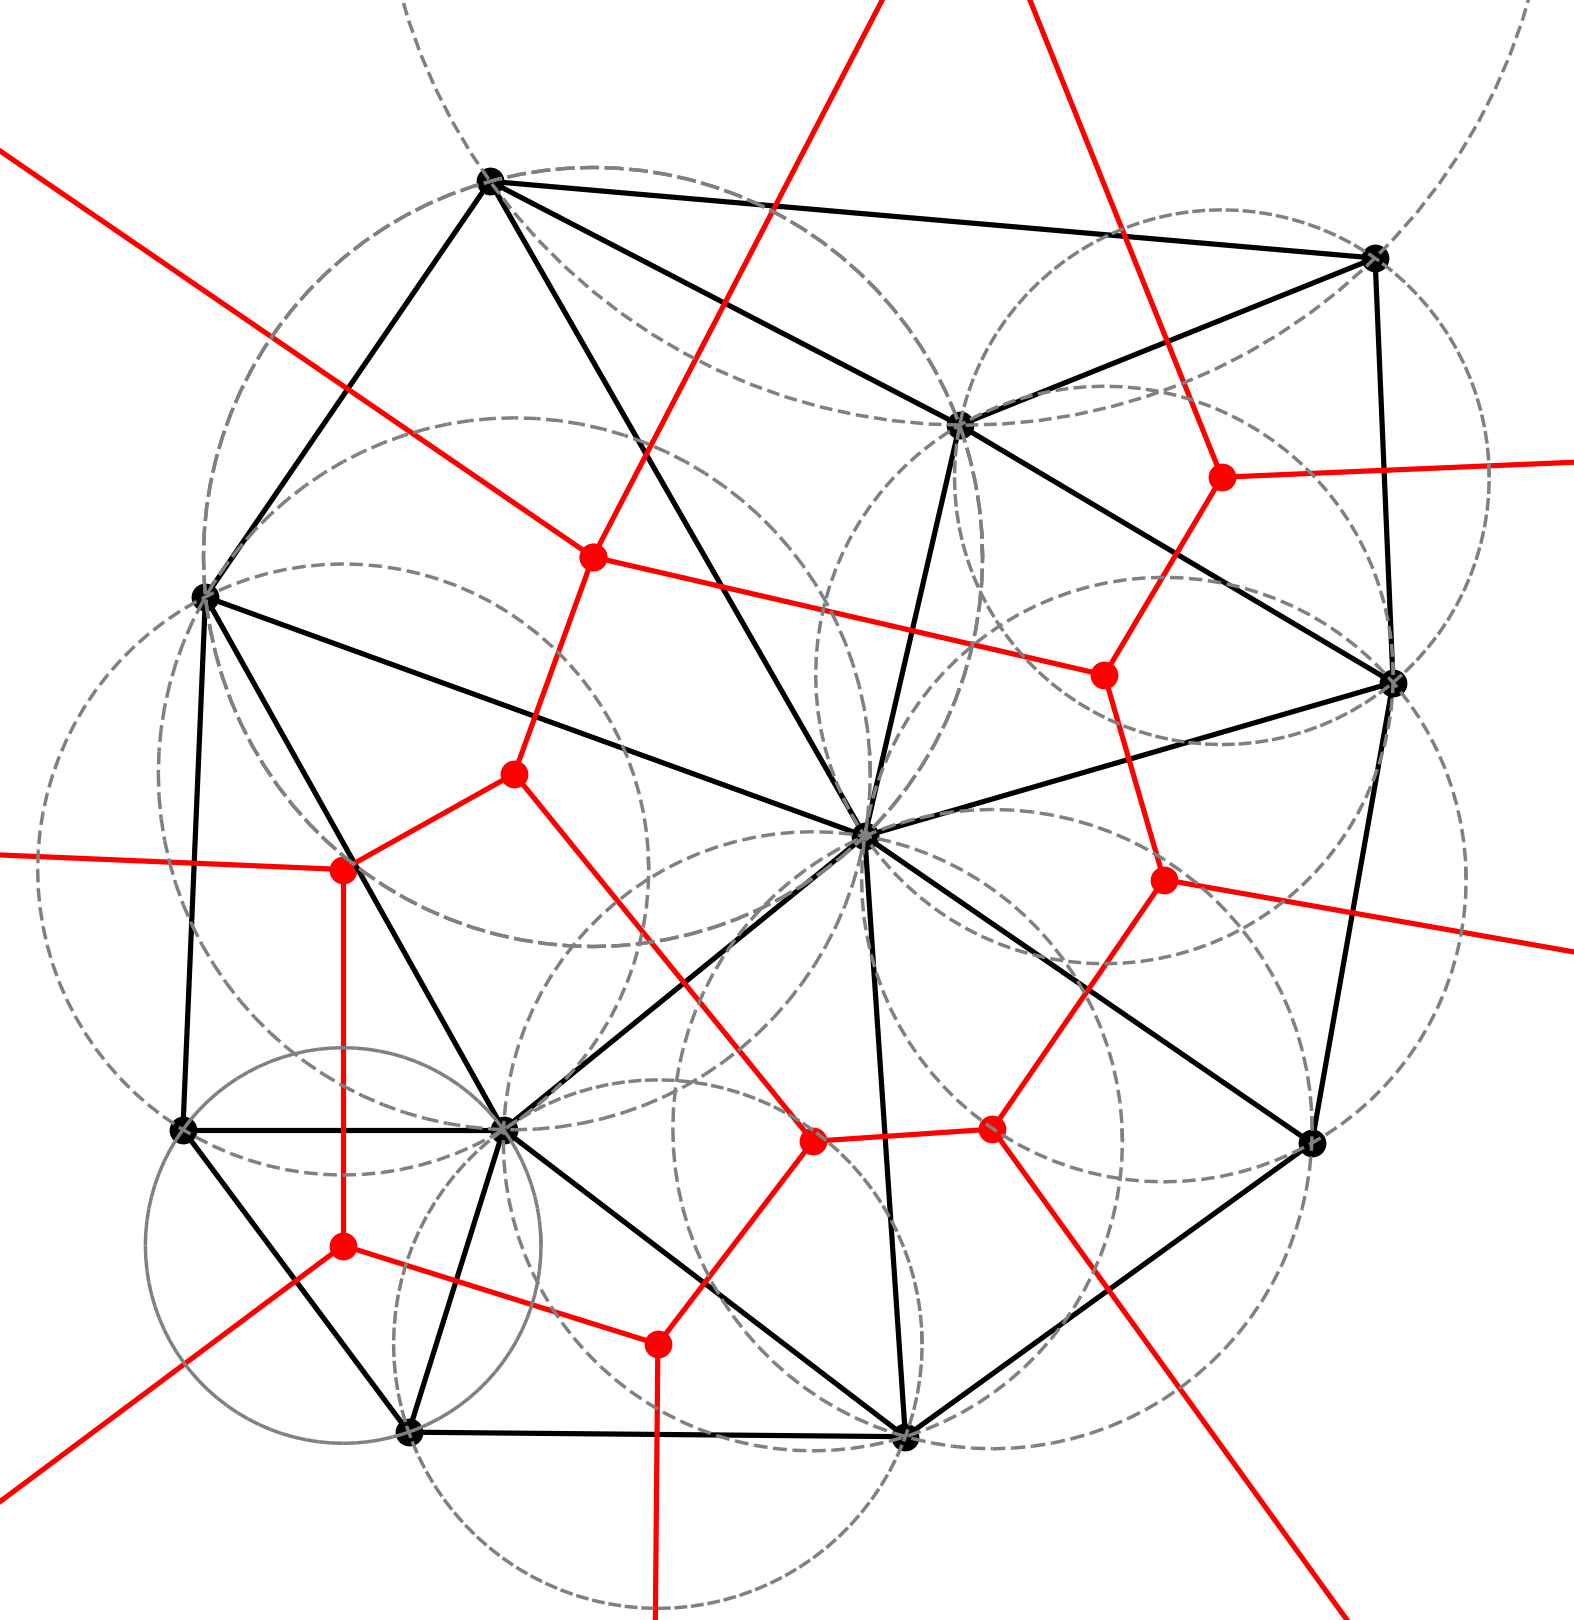
\includegraphics[width=\textwidth]{figs/voronoi1.png}
        \caption{Wprowadzony za pomocą myszki zbiór punktów}
    \end{subfigure}
    \hfill
    \begin{subfigure}[b]{0.3\textwidth}
        \centering
        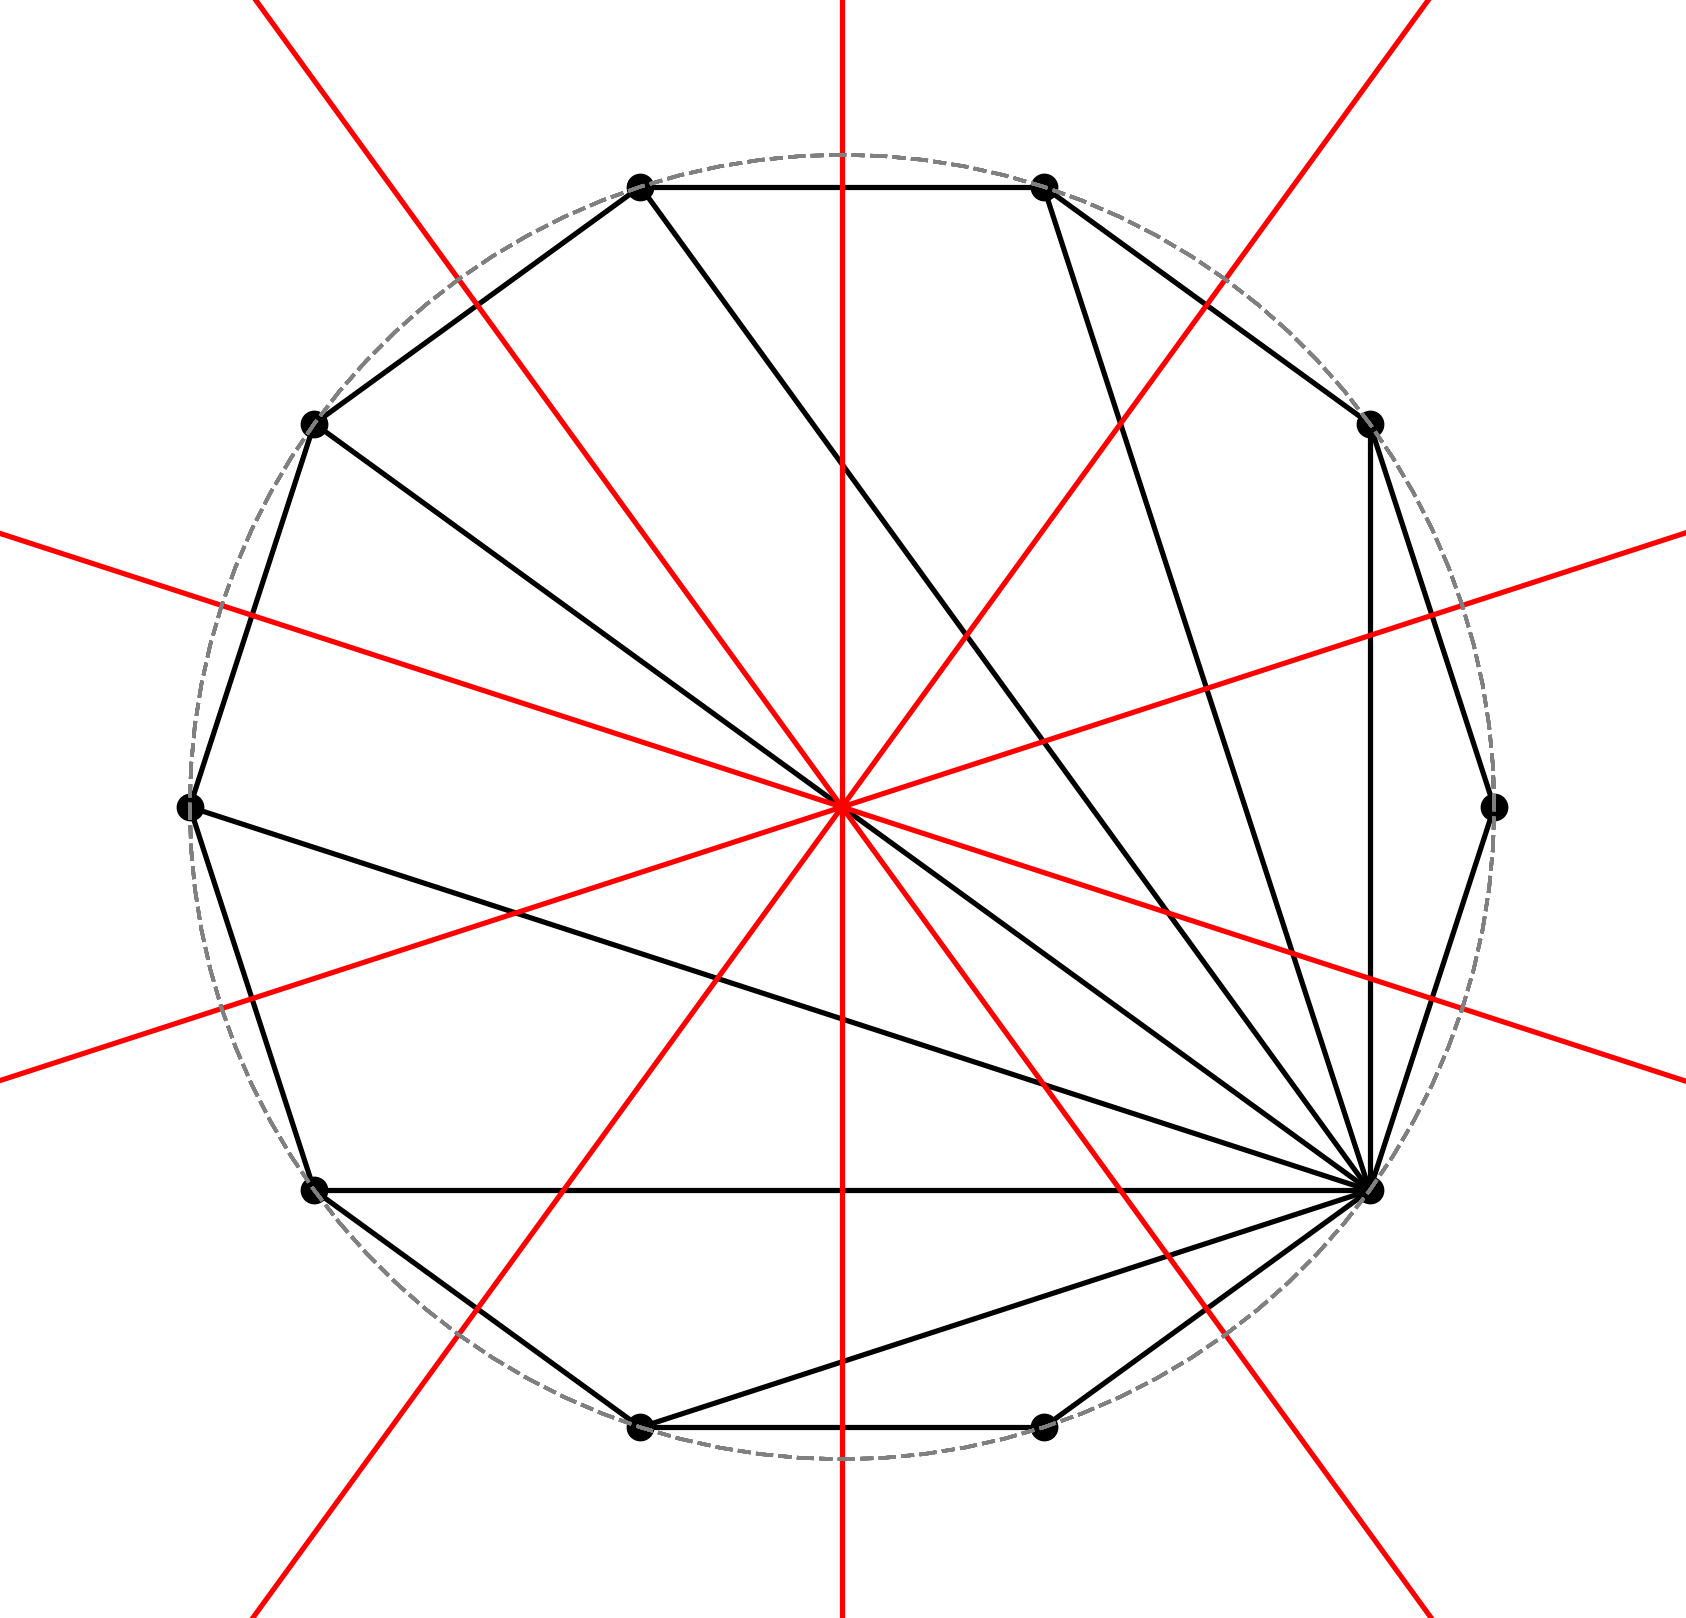
\includegraphics[width=\textwidth]{figs/voronoi2.png}
        \caption{Zbiór punktów będący 10-kątem foremnym}
    \end{subfigure}
    \hfill
    \begin{subfigure}[b]{0.3\textwidth}
        \centering
        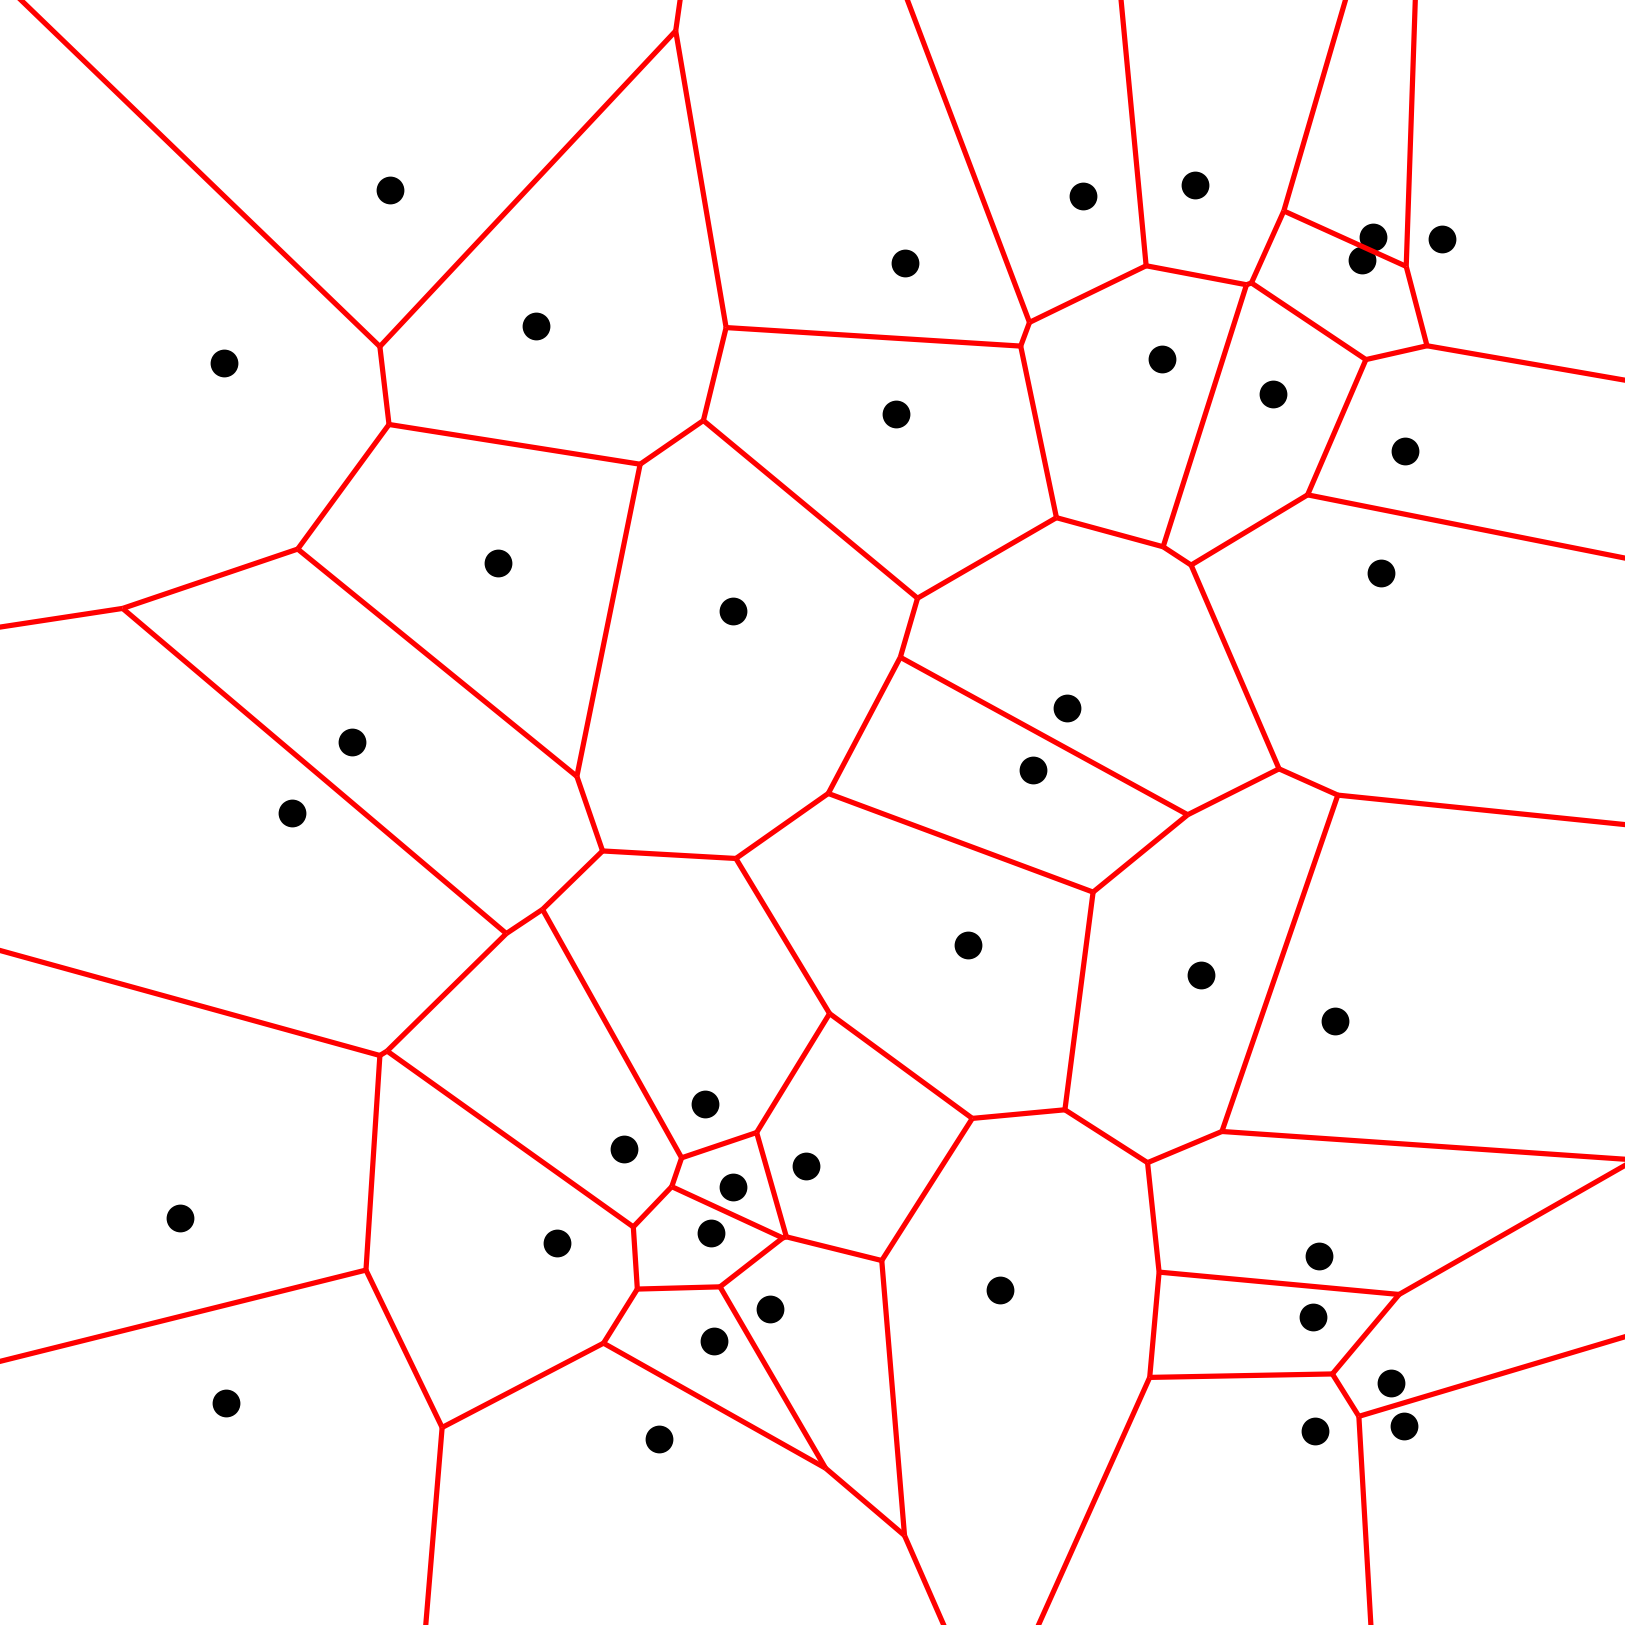
\includegraphics[width=\textwidth]{figs/voronoi3.png}
        \caption{Zbiór 40 wygenerowanych losowo punktów}
    \end{subfigure}

    \caption{Wizualizacja diagramu Woronoja dla trzech różnych zbiorów punktów}
    \label{fig1}
\end{figure}

Zaimplementowany algorytm przetestowano na różnych zbiorach punktów. W
szczególności sprawdzono, czy w przypadku zbioru punktów, dla których więcej niż
3 z nich leżą na jednym okręgu nie występują problemy związane z testem
przynależności do koła opisanego. Nie stwierdzono występowania żadnych problemów
i jak widać na zamieszczonym przykładzie: dla 10-kąta foremnego triangulacja
Delaunay'a i diagram Woronoja zostały wyznaczone poprawnie.

\subsubsection{Wizualizacja etapów działania algorytmu}

Pierwsza część wizualizacji prezentuje algorytm wyznaczania triangulacji
Delaunay'a zadanej chmury punktów, natomiast druga -- przekształcenie uzyskanej
triangulacji w dualny do niej diagram Woronoja. Na Rysunku \ref{fig2}
zamieszczono wybrane fragmenty wizualizacji algorytmu wraz z opisem.

\begin{figure}[ht]
    \centering
    \begin{subfigure}[b]{0.3\textwidth}
        \centering
        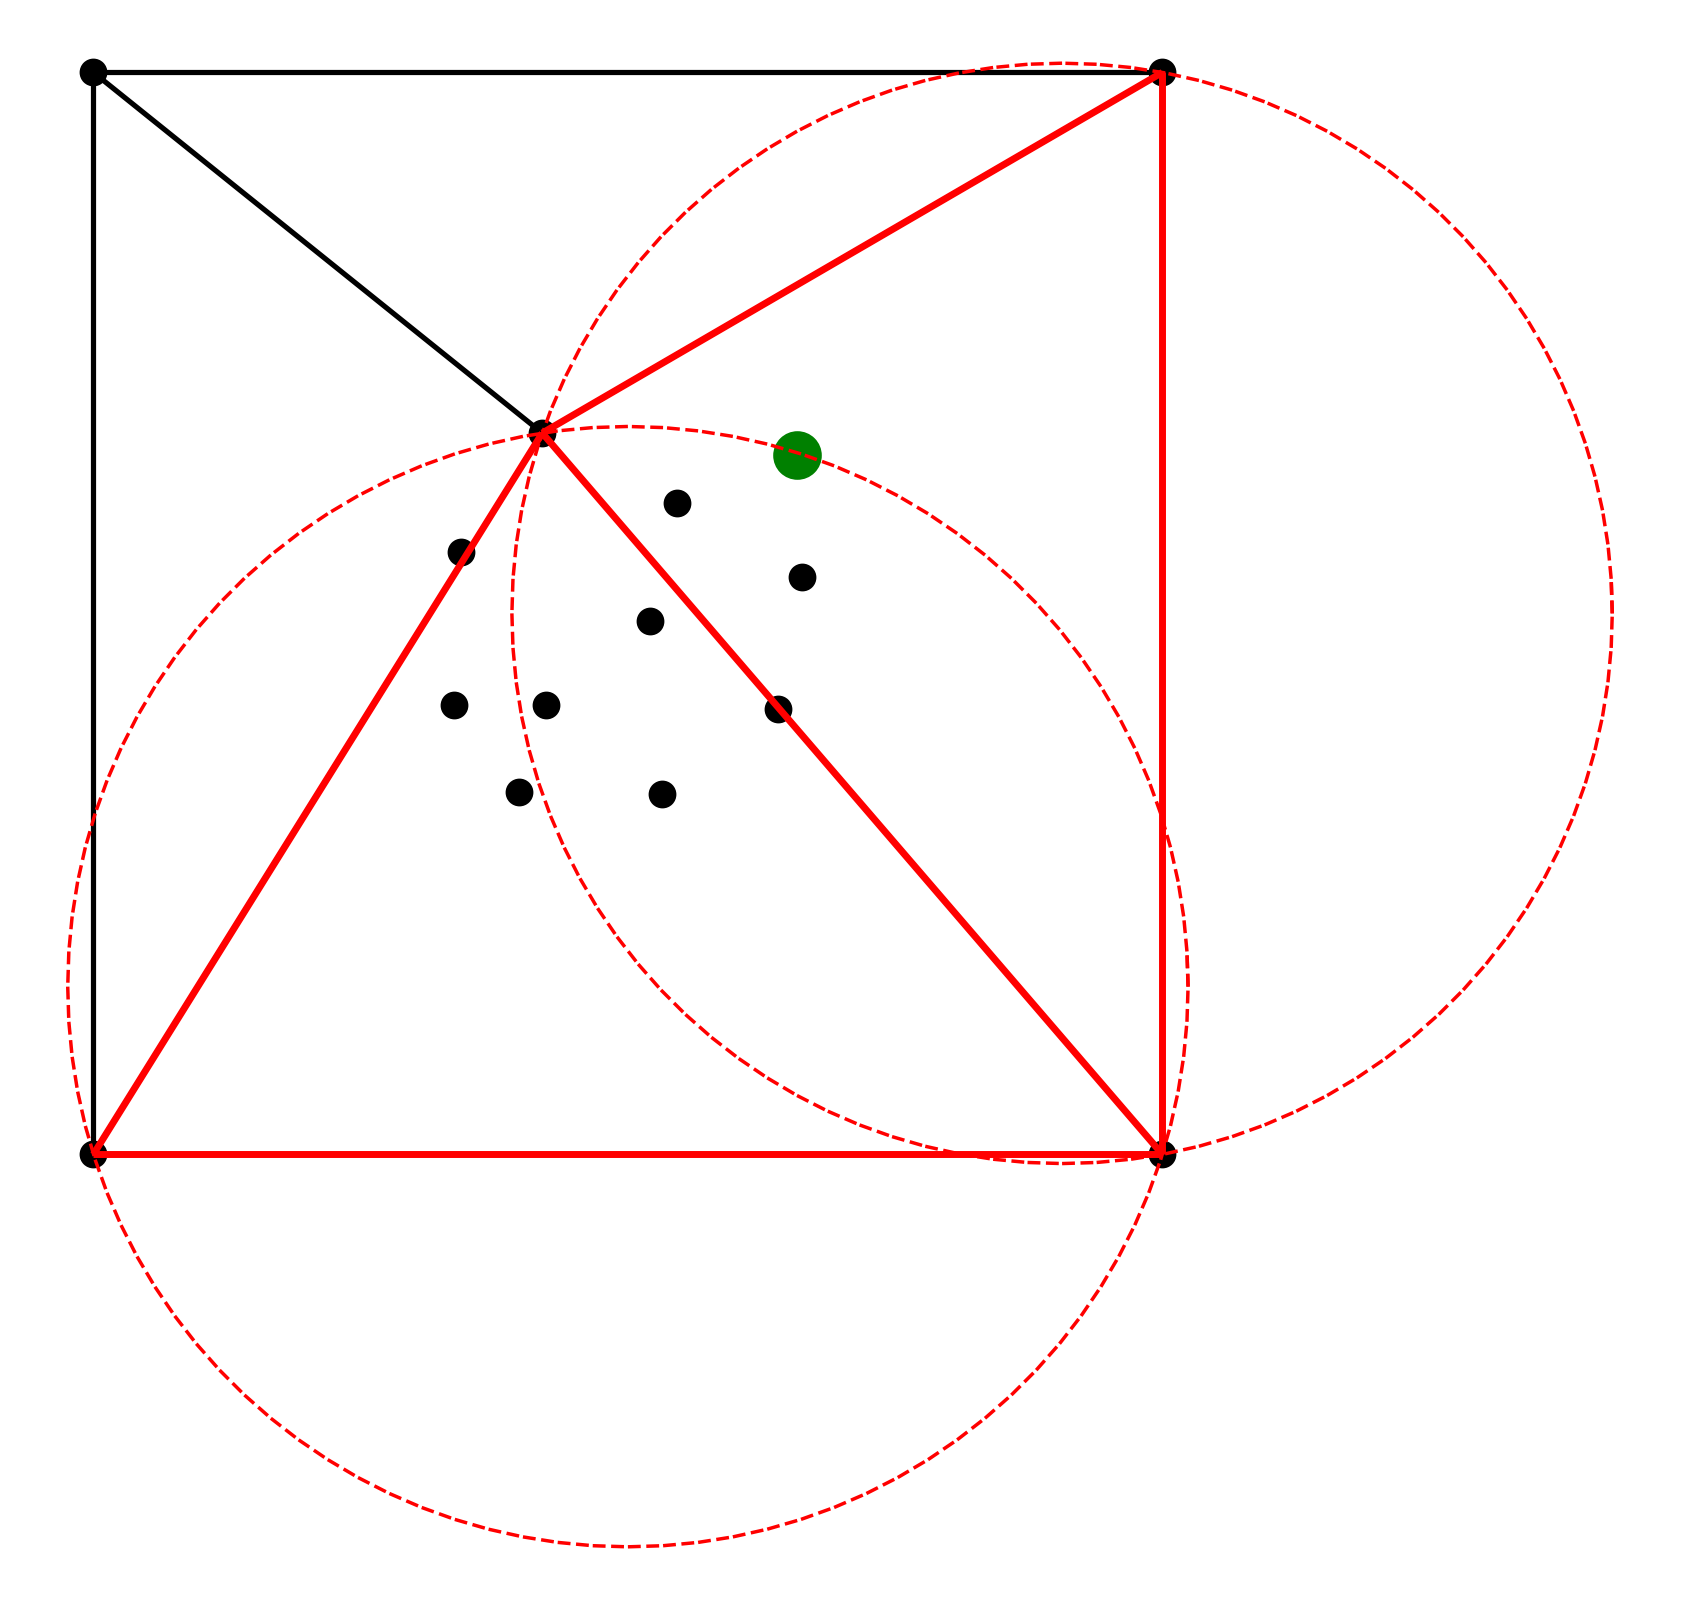
\includegraphics[width=\textwidth]{figs/visual2.png}
        \caption{Znalezienie trójkątów, których okręgi opisane zawierają aktualnie rozpatrywany punkt zaznaczony kolorem zielonym}
    \end{subfigure}  
    \hfill
    \begin{subfigure}[b]{0.3\textwidth}
        \centering
        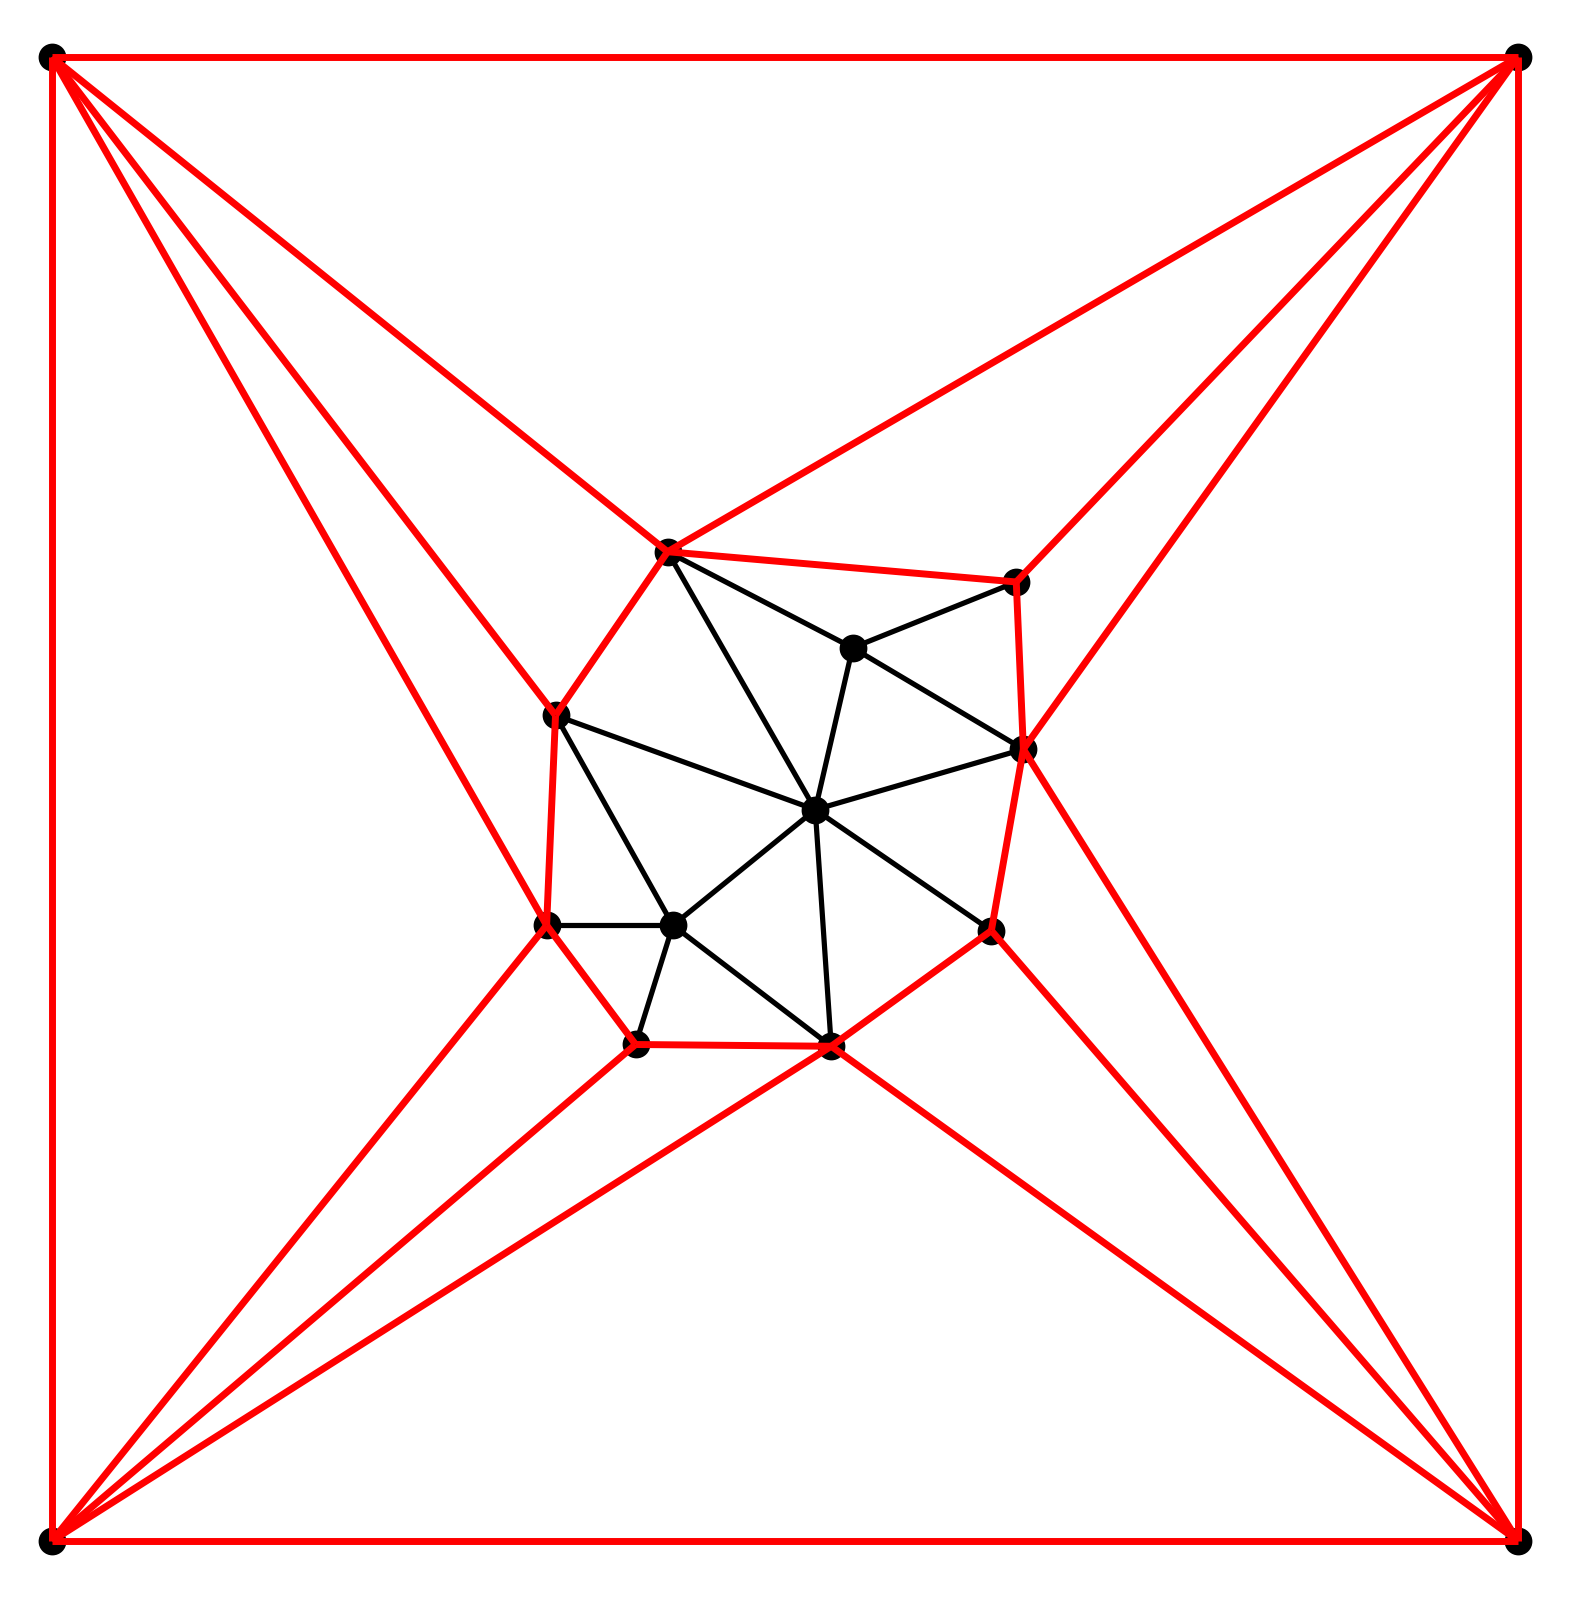
\includegraphics[width=\textwidth]{figs/visual5.png}
        \caption{Usunięcie trójkątów zawierających wierzchołek początkowego superprostokąta}
    \end{subfigure}
    \hfill
    \begin{subfigure}[b]{0.3\textwidth}
        \centering
        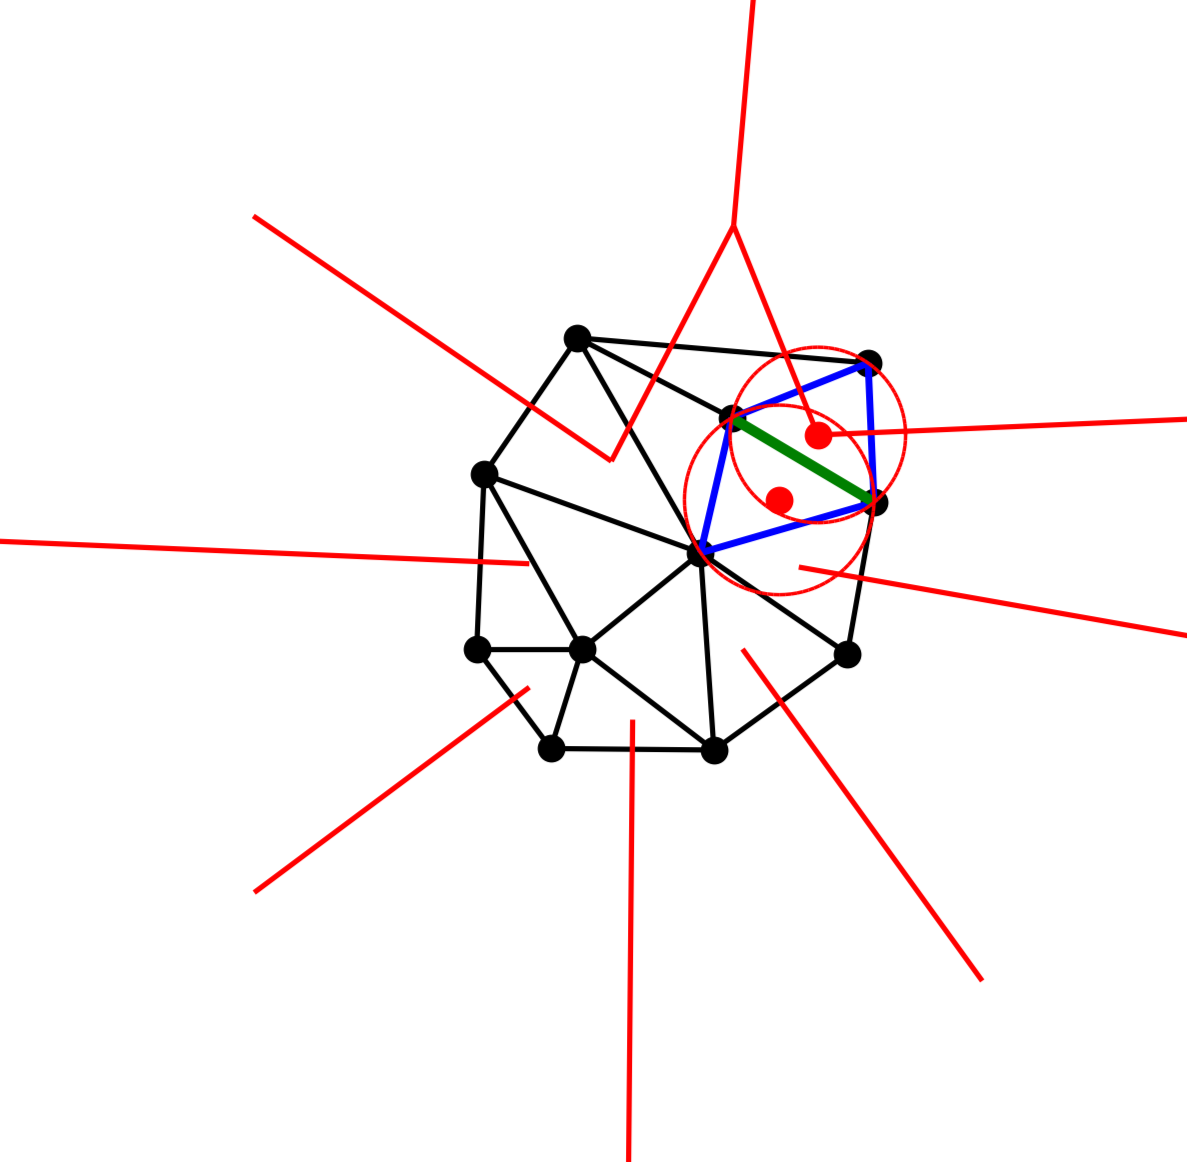
\includegraphics[width=\textwidth]{figs/visual6.png}
        \caption{Utworzenie krawędzi diagramu Woronoja przez połączenie środków okręgów opisanych na trójkątach triangulacji posiadających wspólny bok}
    \end{subfigure}

    \caption{Wybrane fragmenty wizualizacji etapów algorytmu}
    \label{fig2}
\end{figure}

\subsection{Algorytm przybliżony brute force}

\subsubsection{Opis algorytmu}

Jako drugą metodę zaimplementowano algorytm brute force wyznaczający w
przybliżony sposób wieloboki Woronoja dla zadanej chmury punktów. Algorytm
wprowadza na płaszczyźnie dyskretną kratę \(\mathbb{Z}_+^2\)  i dla każdego
punktu kratowego znajduje punkt z zadanej chmury, dla którego odległość (w
sensie metryki euklidesowej) jest minimalna. Algorytm zaimplementowany w języku
Python jest niezwykle krótki, dlatego zamieszczono go poniżej w całości.

\begin{small}
    \begin{lstlisting}[language=python, frame=single]
def ApproxVoronoi(points, N): # O(n*N^2)
    n = len(points)
    P = [i for i in range(n)]
    mx, my = min(points, key=lambda x: x[0])[0], min(points, key=lambda x: x[1])[1]
    Mx, My = max(points, key=lambda x: x[0])[0], max(points, key=lambda x: x[1])[1]
    a = .15 * max(Mx - mx, My - my)
    mx -= a
    my -= a
    Mx += a
    My += a
    hx, hy = (Mx - mx) / N, (My - my) / N
    grid = [[min(P, key=lambda x: d(points[x], (mx+i*hx, my+j*hy))) for j in    
            range(N)] for i in range(N)]

    return grid, mx, my, hx, hy
        \end{lstlisting}
\end{small}

Krata jest reprezentowana przez tablicę dwuwymiarową \(\texttt{grid}[N][N]\),
której wartościami są indeksy punktów z zadanej chmury \texttt{points}. Liczba
naturalna \(N^2\) określa liczbę punktów kratowych i jednocześnie wpływa
bezpośrednio na dokładność wyznaczonego podziału. Obszar, dla którego
wprowadzana jest krata, jest ograniczany do prostokąta
\(((m_x,m_y),(m_x,M_y),(M_x,M_y),(M_x,m_y))\), gdzie \(m_x\), \(m_y\), \(M_x\),
\(M_y\) to odpowiednio przeskalowane minimalne i maksymalne współrzędne punktów
zadanej chmury. Odległość między sąsiednimi punktami kratowymi wynosi wówczas
\(h_x = (M_x-m_x)/N\) (w poziomie) i \(h_y = (M_y-m_y)/N\) (w pionie). Złożoność
czasowa działania tego algorytmu to \(O(nN^2)\), czyli dla ustalonej liczby
punktów kratowych jest liniowa względem wielkości wprowadzonej chmury punktów.

\subsubsection{Graficzna prezentacja wyników działania algorytmu}

Na Rysunku \ref{fig3} przedstawiono wygenerowaną za pomocą algorytmu
aproksymacyjnego dla \(10^4\) punktów kratowych wizualizację diagramu Woronoja
dla 40 losowo wygenerowanych punktów oraz diagram dokładny wyznaczony opisanym
wcześniej algorytmem Bowyera--Watsona.

\begin{figure}[ht]
    \centering
    \hfil
    \begin{subfigure}[b]{0.45\textwidth}
        \centering
        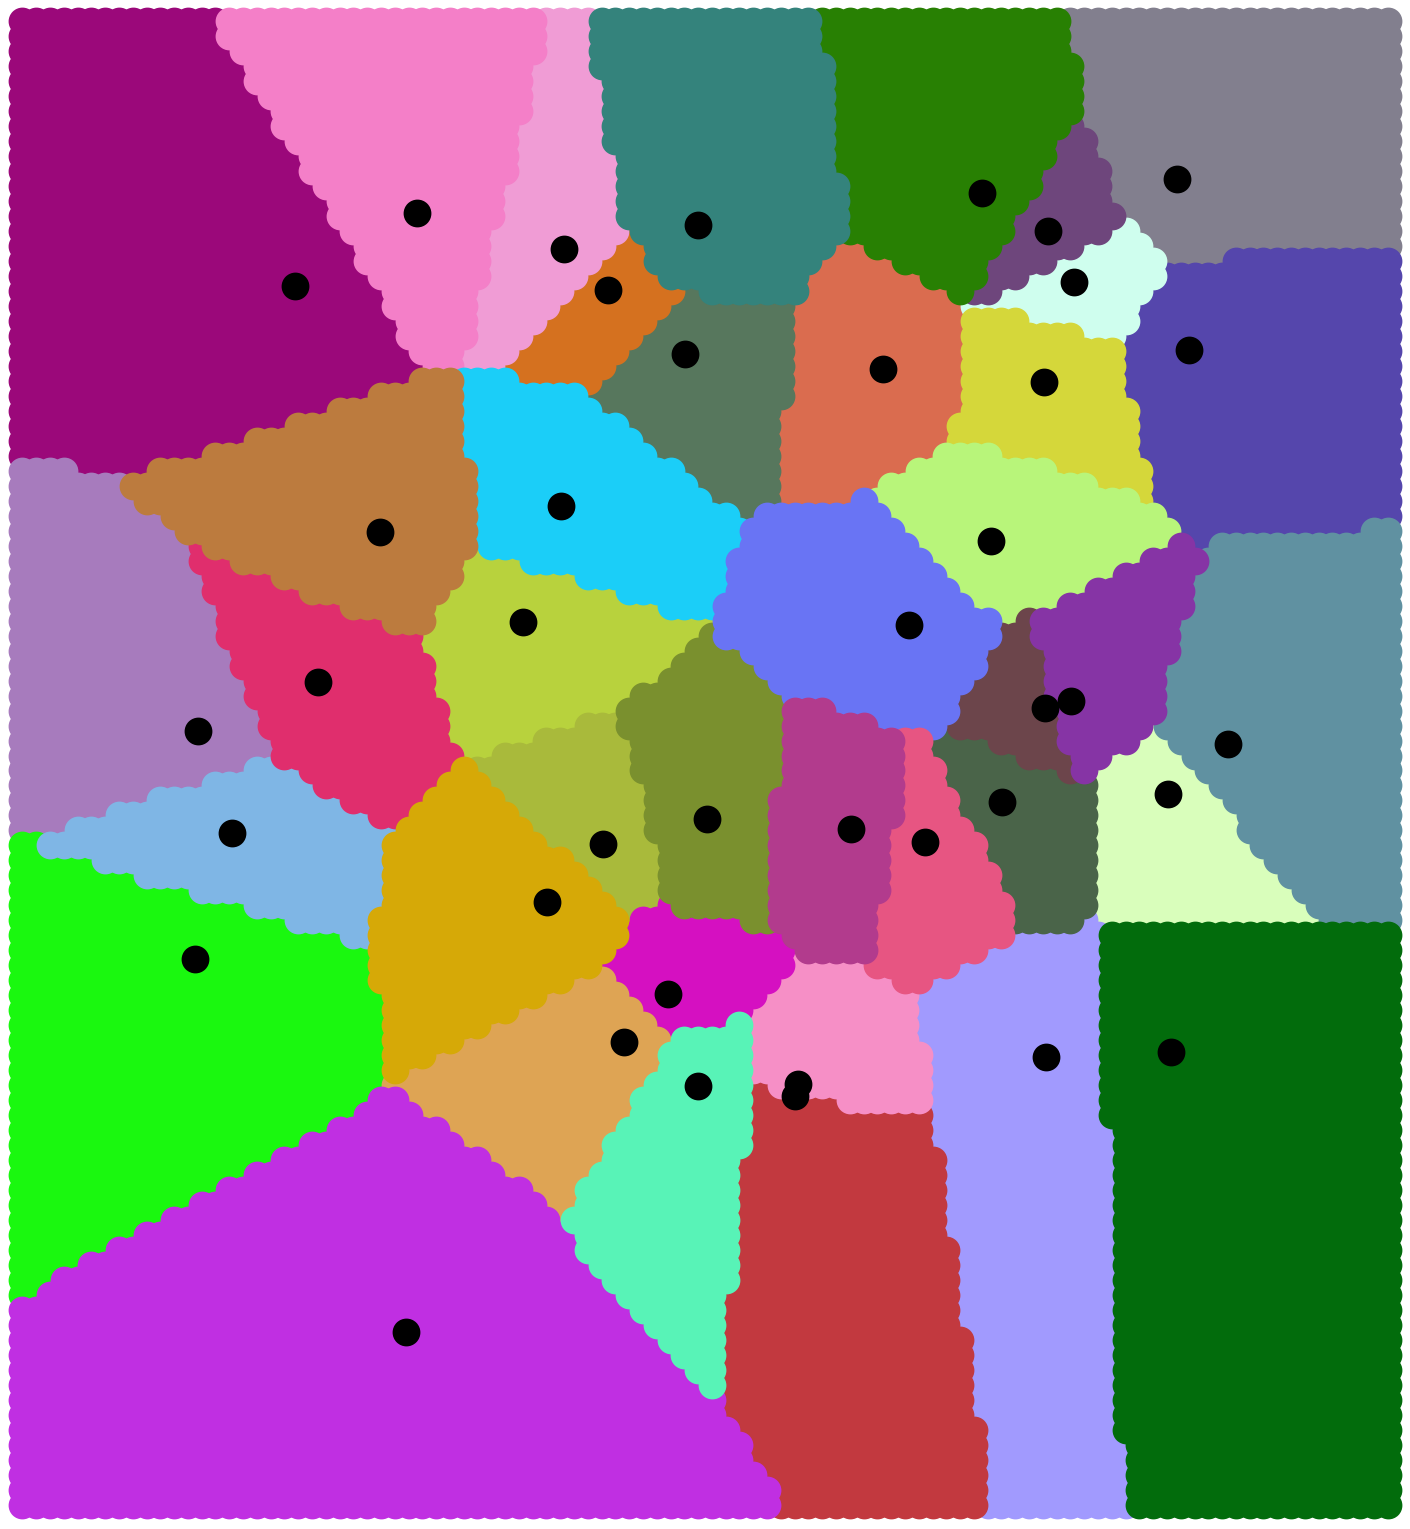
\includegraphics[width=\textwidth]{figs/approx.png}
    \end{subfigure}
    \hfil
    \begin{subfigure}[b]{0.45\textwidth}
        \centering
        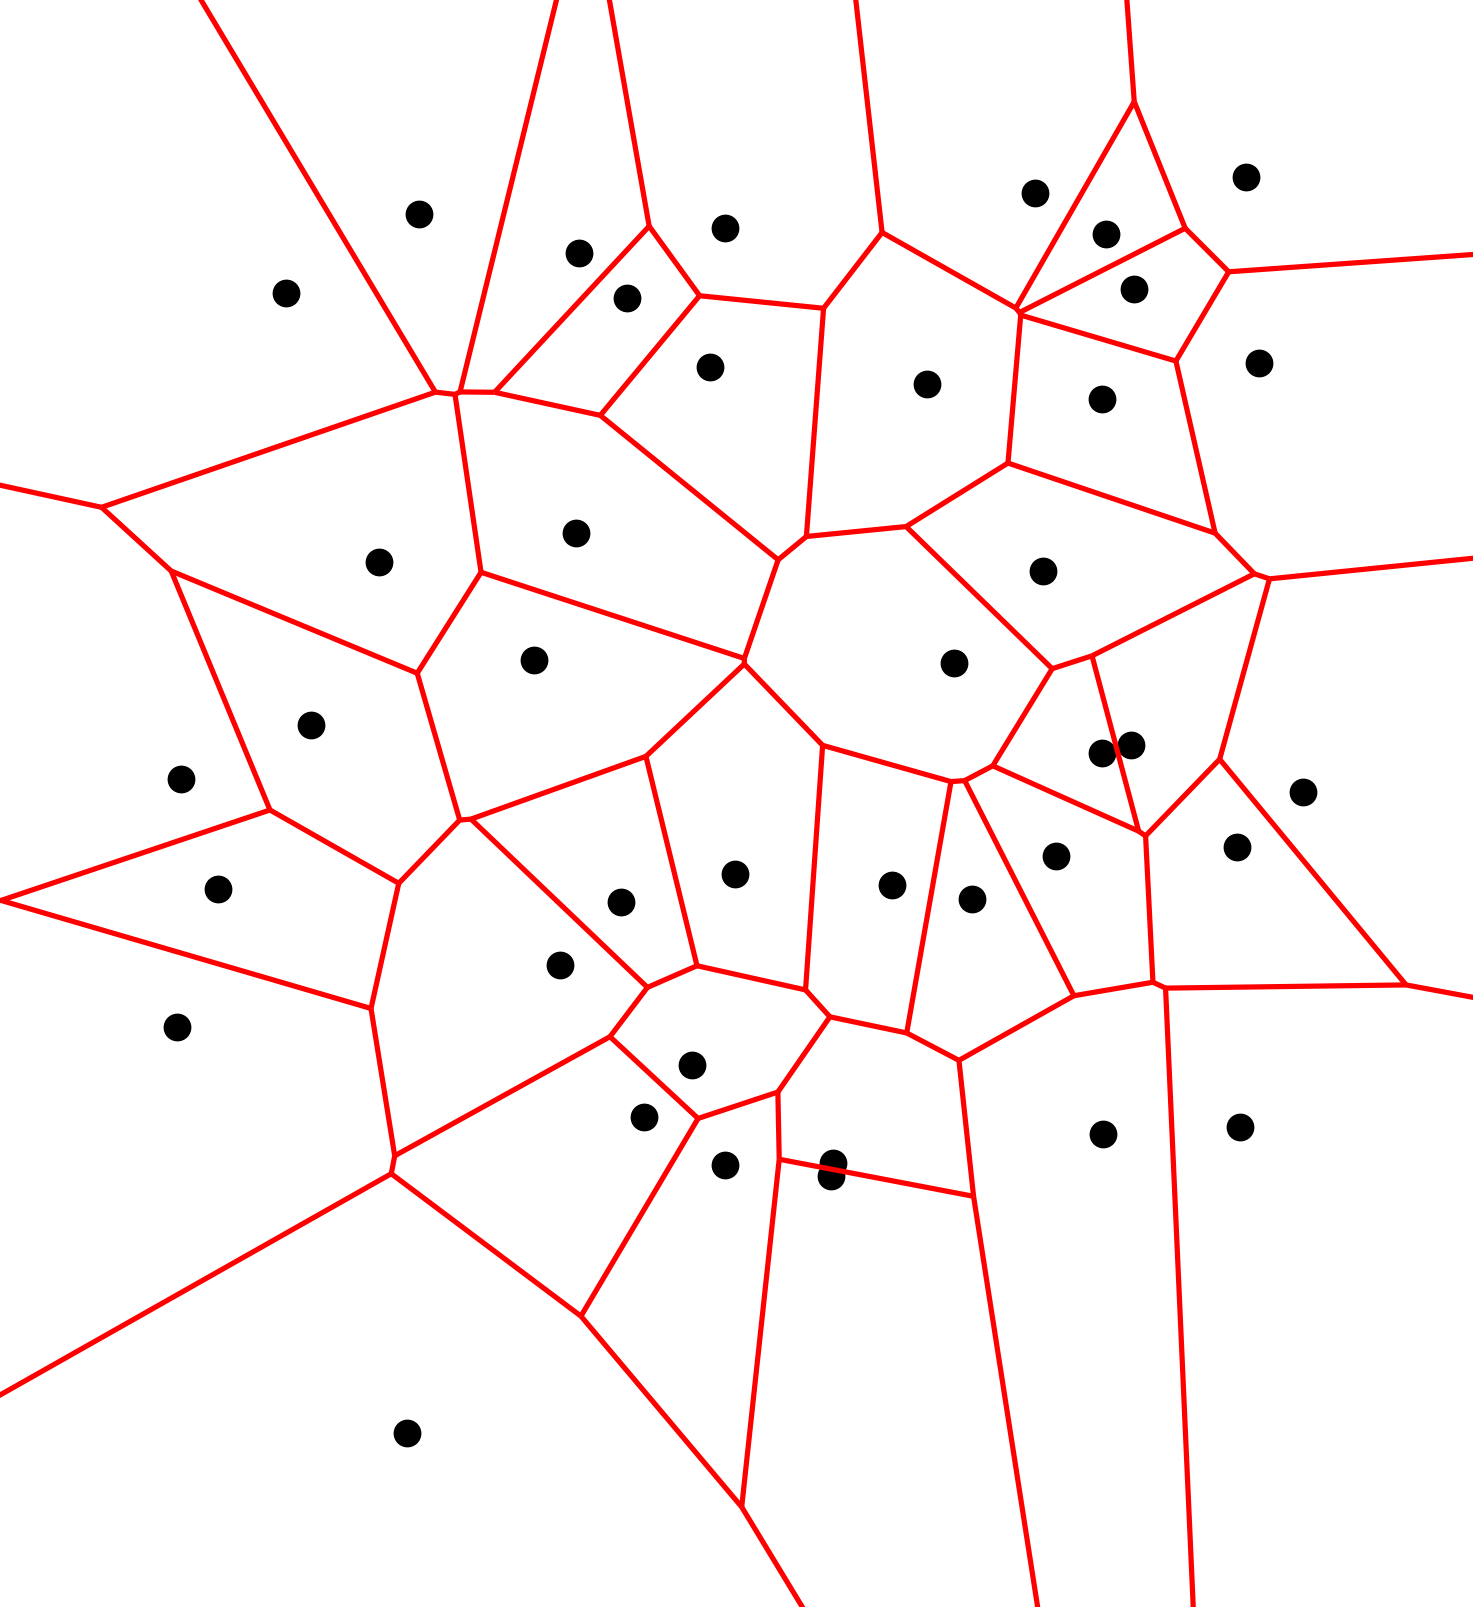
\includegraphics[width=\textwidth]{figs/approx1.png}
    \end{subfigure}
    
    \caption{Przybliżony diagram Woronoja 40 losowych punktów wyznaczony algorytmem aproksymacyjnym dla \(10^4\) punktów kratowych oraz diagram dokładny wyznaczony algorytmem Bowyera--Watsona}
    \label{fig3}

\end{figure}


\end{document}